\documentclass{article}
\usepackage{amsmath}
\usepackage{amssymb}
\usepackage{pgf,tikz}
\title{Principal Component Analysis (PCA)}
\date{2018-02-21}
\author{Kevin Nguyen, MatchCraft LLC}

\begin{document}
\maketitle

\section{Matrix}
\subsection{Definition}
Let X be d x n matrix where d is number of rows and n is number of columns.

$$
X =
\begin{bmatrix}
  x_{11} & x_{12} & x_{13} & \dots & x_{1n} \\
  x_{21} & x_{22} & x_{13} & \dots & x_{2n} \\
  \vdots & \vdots & \vdots & \ddots & \vdots \\
  x_{d1} & x_{d2} & x_{d3} & \dots & x_{dn} \\
\end{bmatrix}
=
\begin{pmatrix}
  x_{11} & x_{12} & x_{13} & \dots & x_{1n} \\
  x_{21} & x_{22} & x_{13} & \dots & x_{2n} \\
  \vdots & \vdots & \vdots & \ddots & \vdots \\
  x_{d1} & x_{d2} & x_{d3} & \dots & x_{dn} \\
\end{pmatrix}
= (x_{ij}) \in \mathbb{R}^{d \times n}
$$

\subsection{Transpose}

$$
X^T = 
\begin{bmatrix}
  x_{11} & x_{21} & x_{31} & \dots & x_{d1} \\
  x_{12} & x_{22} & x_{32} & \dots & x_{d2} \\
  \vdots & \vdots & \vdots & \ddots & \vdots \\
  x_{1n} & x_{2n} & x_{3n} & \dots & x_{dn} \\
\end{bmatrix}
=
\begin{pmatrix}
  x_{11} & x_{21} & x_{31} & \dots & x_{d1} \\
  x_{12} & x_{22} & x_{32} & \dots & x_{d2} \\
  \vdots & \vdots & \vdots & \ddots & \vdots \\
  x_{1n} & x_{2n} & x_{3n} & \dots & x_{dn} \\
\end{pmatrix}
= (x_{ji}) \in \mathbb{R}^{n \times d}
$$

\subsection{Matrix Multiplication}
If X is d x n matrix and Y is n x m matrix, then XY is d x m matrix. $XY_{ij}$ is the value of row i column j of matrix XY.

$$XY_{ij} = x_{i1}y_{1j} + x_{i2}y_{2j} + x_{i3}y_{3j} + \dots x_{in}y_{nj} = \sum_{k=1}^{n}x_{ik}y_{kj}$$

$$
S
= XX^T
=
\begin{bmatrix}
  x_{11} & x_{12} & \dots & x_{1n} \\
  x_{21} & x_{22} & \dots & x_{2n} \\
  \vdots & \vdots & \ddots & \vdots \\
  x_{d1} & x_{d2} & \dots & x_{dn} \\
\end{bmatrix}
\begin{bmatrix}
  x_{11} & x_{21} & \dots & x_{d1} \\
  x_{12} & x_{22} & \dots & x_{d2} \\
  \vdots & \vdots & \ddots & \vdots \\
  x_{1n} & x_{2n} & \dots & x_{dn} \\
\end{bmatrix}
\\
=
\begin{bmatrix}
  X_{1}X_{1}^T & X_{1}X_{2}^T & \dots & X_{1}X_{d}^T \\
  X_{2}X_{1}^T & X_{2}X_{2}^T & \dots & X_{2}X_{d}^T \\  
  \vdots & \vdots  & \ddots & \vdots \\
  X_{d}X_{1}^T & X_{d}X_{2}^T & \dots & X_{d}X_{d}^T \\  
\end{bmatrix}
$$

\section{Vectors}
Let \textbf{x} and \textbf{u} vector vector of d dimension. The projection of \textbf{x} onto \textbf{u} is

\begin{center}
  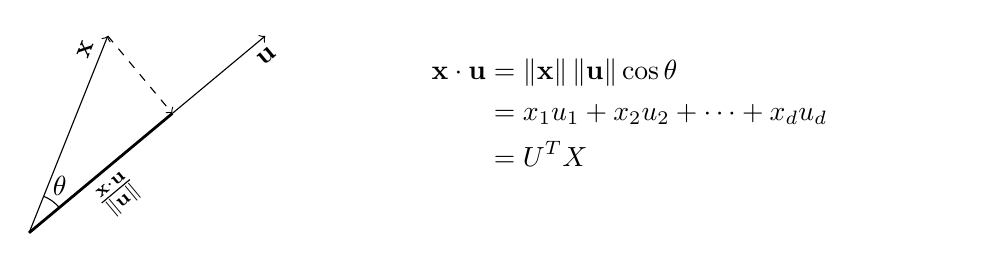
\begin{tikzpicture}[scale=.5]
    \coordinate (origin) at (0,0);
  \draw[->] (0,0) -- (2,5) node (u) [pos=.9,sloped, above]{$\mathbf{x}$};
  \draw[line width=1pt] (0, 0) -- (3.639344262295082, 3.0327868852459017) node (proj_u) [pos=.5,sloped, below]{$\frac{\mathbf{x} \cdot \mathbf{u}}{\left \| \mathbf{u} \right \|}$};
  \draw[->] (3.639344262295082, 3.0327868852459017) -- (6,5) node (u) [pos=.9,sloped, below]{$\mathbf{u}$};
  \draw[dashed, ->] (2,5) -- (3.639344262295082, 3.0327868852459017);
  \draw (0.7682212795973759, 0.6401843996644798) arc (39.8055710922652:68.1985905:1) node at (.78,1.2) {$\theta$};

  \node [right=1cm,text width=8cm] at (5,3) {
    $$
    \begin{aligned}
      \mathbf{x} \cdot \mathbf{u} &= \left \| \mathbf{x} \right \| \left \| \mathbf{u} \right \| \cos \theta \\
      &= x_1 u_1 + x_2 u_2 + \dots + x_d u_d \\        
      &= U^{T}X
    \end{aligned}
    $$
  };
\end{tikzpicture}
\end{center}

\section{Lagrange Multipliers}

\section{Variance}
\subsection{Variance}

Let X be a dataset of size n:

$$X = [x_1, x_2, ..., x_n]$$

Mean of X is
$$E[X] = \mu = \frac{1}{n}\sum_{i=1}^{n}x_i$$
Variance of X is the average of square distance from the mean.
$$Var(X) = \sigma^2 = \frac{1}{n}\sum_{i=1}^{n} (x_i - \mu)^2$$

If we shift X to center around its mean then

$$Var(X)
= \frac{1}{n}\sum_{i=1}^{n}(x_i)^2
=
\begin{pmatrix}
  x_1 & x_2 & x_3 & \dots & x_n \\
\end{pmatrix}
\begin{pmatrix}
  x_1 \\ x_2 \\ x_3 \\ \vdots x_n\\
\end{pmatrix}
= \mathbf{XX}^T
$$

\section{Intuition}
Let X be a dataset of size n:
$$ X = [\mathbf{x}_1, \mathbf{x}_2, ..., \mathbf{x}_n] where \mathbf{x}  $$

\end{document}
